\documentclass{beamer}

\mode<presentation> {

% The Beamer class comes with a number of default slide themes
% which change the colors and layouts of slides. Below this is a list
% of all the themes, uncomment each in turn to see what they look like.

%\usetheme{default}
%\usetheme{AnnArbor}
%\usetheme{Antibes}
%\usetheme{Bergen}
%\usetheme{Berkeley}
%\usetheme{Berlin}
%\usetheme{Boadilla}
%\usetheme{CambridgeUS}
%\usetheme{Copenhagen}
%\usetheme{Darmstadt}
%\usetheme{Dresden}
%\usetheme{Frankfurt}
%\usetheme{Goettingen}
%\usetheme{Hannover}
%\usetheme{Ilmenau}
%\usetheme{JuanLesPins}
%\usetheme{Luebeck}
%\usetheme{Madrid}
%\usetheme{Malmoe}
%\usetheme{Marburg}
%\usetheme{Montpellier}
%\usetheme{PaloAlto}
\usetheme{Pittsburgh}
%\usetheme{Rochester}
%\usetheme{Singapore}
%\usetheme{Szeged}
%\usetheme{Warsaw}

% As well as themes, the Beamer class has a number of color themes
% for any slide theme. Uncomment each of these in turn to see how it
% changes the colors of your current slide theme.

%\usecolortheme{albatross}
%\usecolortheme{beaver}
%\usecolortheme{beetle}
%\usecolortheme{crane}
%\usecolortheme{dolphin}
%\usecolortheme{dove}
%\usecolortheme{fly}
%\usecolortheme{lily}
%\usecolortheme{orchid}
%\usecolortheme{rose}
%\usecolortheme{seagull}
%\usecolortheme{seahorse}
%\usecolortheme{whale}
%\usecolortheme{wolverine}

%\setbeamertemplate{footline} % To remove the footer line in all slides uncomment this line
%\setbeamertemplate{footline}[page number] % To replace the footer line in all slides with a simple slide count uncomment this line

%\setbeamertemplate{navigation symbols}{} % To remove the navigation symbols from the bottom of all slides uncomment this line
}

\usepackage{graphicx}
\usepackage{booktabs}


\title[Short title]{Non-zero-sum Game and Nash Equilibarium}

\author{Team nogg}
\institute[SJTU]
{

}
\date{\today}

\begin{document}

\begin{frame}
\titlepage
\end{frame}

\begin{frame}
\frametitle{Overview}
\tableofcontents
\end{frame}


\section{Nash’s Theorem}
\begin{frame}{Nash's Theorem}
	\begin{itemize}[]
		\item \textbf{\large Nash's Theorem}:
		
		\qquad Every game with a finite number of players and a finite number of actions
		available to each player has a Nash equilibrium.
	\end{itemize}
\end{frame}

\begin{frame}[fragile]{How to prove it?}
\begin{itemize}[<+->]
	\item Nash's original proof of it used \textbf{Kakutani's fixed point theorem}.
	\item But a year later Nash simplified his proof to only use \textbf{Brouwer’s fixed point theorem}.
\end{itemize}
\end{frame}

\begin{frame}[fragile]{How to prove it?}
	\begin{itemize}
		\item Nash's original proof of it used \textbf{Kakutani's fixed point theorem}.
		\item But a year later Nash simplified his proof to only use \textbf{\color{red}\large Brouwer’s fixed point theorem}.
	\end{itemize}
\end{frame}

\begin{frame}[fragile]{Brouwer’s fixed point theorem}
	\begin{itemize}
		\item \textbf{\large Brouwer’s fixed point theorem}:
		
		\qquad Let $D$ be a convex, compact subset of the Euclidean space. If $f : D\  \overrightarrow{}\ D$ is
		continuous, then there exists $x \in D$ such that $f (x) = x$.
	\end{itemize}
\end{frame}

\begin{frame}[fragile]{Brouwer’s fixed point theorem}
	\begin{itemize}
		\item \textbf{Examples}:
		\begin{itemize}
			\item Take an ordinary map of a country, and suppose that that map is laid out on a table inside that country. There will always be a "You are Here" point on the map which represents that same point in the country.
		\end{itemize}
		\begin{figure}[H]
			\centering
			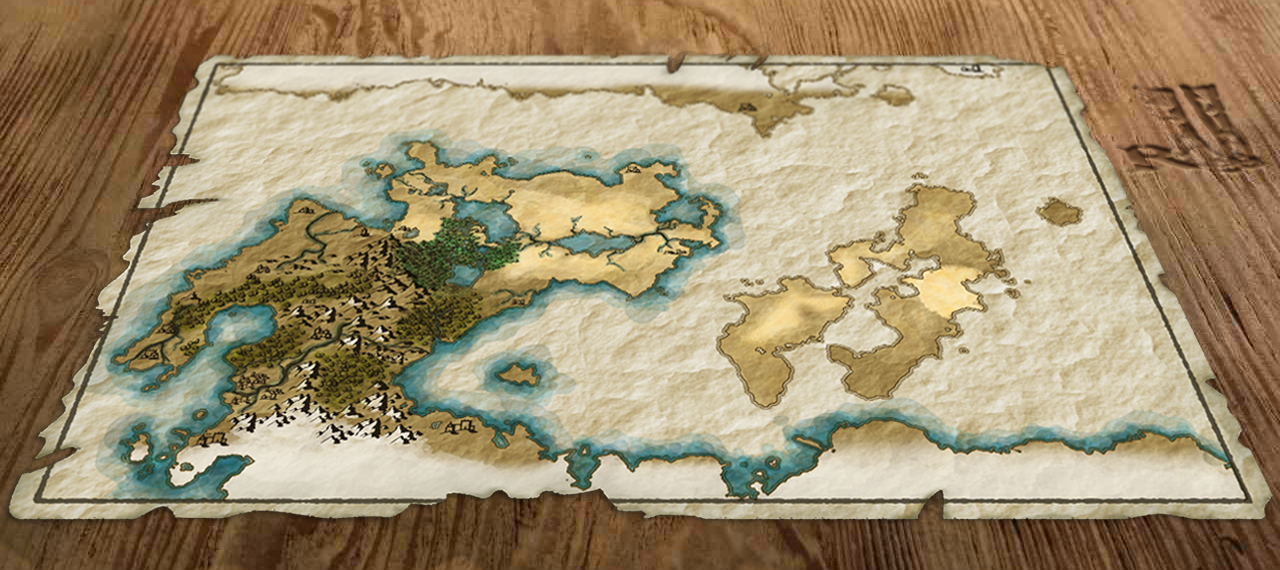
\includegraphics[width=0.7\linewidth]{001.jpg}\vspace{-10pt}
			\nonumber\vspace{-10pt}
		\end{figure}
	\end{itemize}
\end{frame}

\begin{frame}[fragile]{Gain function}
	\begin{itemize}[<+->]
		\item Now we introduce the idea of \textbf{Gain function}:\\
		\begin{equation}
		Gain_{p;s_p} (x) = max\{u_p(s_p;x_{-p})-u_p(x), 0\} \ \  \ \ \ \ \ \nonumber
		\end{equation}
		\item In other words, the $Gain$ is equal to the increase in payoff for player p if he were to switch to pure
		strategy $s_p$.
		\item Obviously, the $Gain$ for all players is 0 in \textbf{Nash Equilibrium}.
	\end{itemize}
\end{frame}

\begin{frame}[fragile]{Proof of Nash' Theorem}
	\begin{itemize}[<+->]
		\item Now we define a function $f$ as follows:
		 \begin{equation}
		 y_p(s_p) := \frac{x_p(s_p) + Gain_{p;s_p}(x)}{1 + \sum_{s'_p \in S_p} Gain_{p;s'_p}(x)} \ \ \ \ \ \ \ \nonumber
		 \end{equation}
		\item In other words, function $f$ tries to boost the probability mass that player p places on various pure strategies
		depending on the $p$ gains in payoff the player would get by switching to these strategies.
	\end{itemize}
\end{frame}

\begin{frame}[fragile]{Proof of Nash' Theorem}
	\begin{itemize}[<+->]
		\item It is easy to see that f is continuous, convex and compact. So we can use \textbf{Brouwer’s fixed point theorem}, there is at least one fixed point of function $f$.
		\item For any fixed point $x=f(x)$, 
		\begin{equation}
		Gain_{p;s_p}(x) = 0, \ \ \  \forall p\in [n], s_p \in S_p .\nonumber
		\end{equation}
	It will be proved later.
	\item Then we claim that any fixed point of $f$ is a \textbf{Nash equilibrium}.
	\end{itemize}
\end{frame}

\begin{frame}[fragile]{Proof of Nash' Theorem}
	\begin{itemize}[<+->]
		\item It is easy to see that f is continuous, convex and compact. So we can use \textbf{Brouwer’s fixed point theorem}, there is at least one fixed point of function $f$.
		\item For any fixed point $x=f(x)$, 
		\begin{equation}
		Gain_{p;s_p}(x) = 0, \ \ \  \forall p\in [n], s_p \in S_p .\nonumber
		\end{equation}
		It can be proved by by contradiction.
		\item Then we claim that any fixed point of $f$ is a \textbf{Nash equilibrium}.
	\end{itemize}
\end{frame}

\begin{frame}[fragile]{The smile of John Nash}
	\begin{figure}[H]
		\centering
		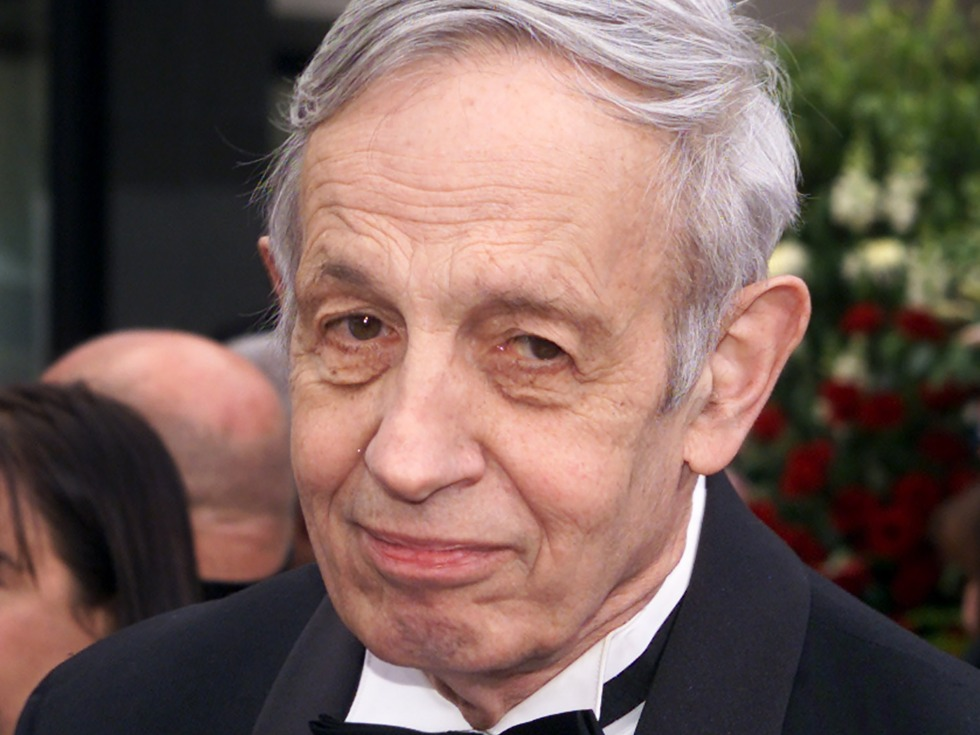
\includegraphics[width=0.7\linewidth]{002.jpeg}\vspace{-10pt}
		\nonumber\vspace{-10pt}
	\end{figure}
\end{frame}


\begin{frame}
\Huge{\centerline{The End}}
\end{frame}


\end{document} 
